% !TEX program = xelatex
\documentclass[UTF8,a4paper,11pt]{ctexart}

\usepackage[a4paper,margin=2.05cm,headheight=14pt]{geometry}
\usepackage{amsmath,amssymb,booktabs,longtable,array,tabularx}
\usepackage{graphicx}
\usepackage{xcolor}
\usepackage{xurl}
\usepackage{hyperref}

\definecolor{pyblue}{RGB}{36,91,163}
\definecolor{qudared}{RGB}{190,65,55}
\hypersetup{
  colorlinks=true,
  linkcolor=pyblue,
  urlcolor=pyblue,
  pdftitle={PyQCU 与 QUDA MultiGrid 全面对比测试报告}
}
\graphicspath{{../data/report_multigrid_comprehensive_20260928/final_protocol/report/}{../data/report_multigrid_comprehensive_20260928/final_protocol/}}
\newcolumntype{L}[1]{>{\raggedright\arraybackslash}p{#1}}
\newcolumntype{Y}{>{\raggedright\arraybackslash}X}
\newcommand{\code}[1]{\texttt{\detokenize{#1}}}
\setlength{\parindent}{2em}
\setlength{\parskip}{0.35em}
\emergencystretch=3em

\title{PyQCU 与 QUDA MultiGrid 全面对比测试报告}
\author{PyQCU 测试记录}
\date{2026 年 9 月 28 日}

\begin{document}
\maketitle

\begin{abstract}
本文记录 PyQCU Strict MultiGrid 与 QUDA 1.1.0 MultiGrid 在 V100
单卡（\code{sm_70}）和双 P100（\code{sm_60}）上的正式笛卡尔测试。
目标矩阵覆盖两种实现、六种精度/格点配置、trace on/off、BiCGStab、
MG-2 与 MG-3，每个可执行单元均执行 1 次 cold、2 次 warmup 和 5 次
steady。精确格点侧记录 132 条 side record，其中 66 个 combined 单元
全部通过配置哈希、输入 bundle、公平性和独立真残差门。双 P100 的
$16\times32\times32\times48$ c64 请求项受 85\% 显存门限和 570 秒
单实例时限约束，明确替代为同精度的 $16^4$ 实例并单独登记，未伪造为
原格点结果。所有原始 JSON、TSV、CSV、SVG 和 PDF 均保存在
\path{data/report_multigrid_comprehensive_20260928/}。
\end{abstract}

\tableofcontents

\section{任务定义与验收标准}

本次测试对象为 \path{pyqcu} 与 \path{refer/git-rep/quda}。测试结果
必须回答以下问题：

\begin{enumerate}
  \item 在相同格点、精度、层级、初始猜测和真残差门下，PyQCU 与 QUDA
        的总 solve 时间、外层迭代数和最细层残差各是多少；
  \item MG 每一层的 pre-smoother、post-smoother、restriction、
        prolongation、coarse solver 和 other 耗时各是多少；
  \item trace on 的诊断开销与 trace off 的正式性能是否被混淆；
  \item V100 单卡和双 P100 的最大显存观测值是否低于设备容量的 85\%；
  \item 若请求实例超过资源或时间门限，替代实例是否被明确记录而不是
        静默跳过。
\end{enumerate}

通过标准为：每个精确单元两侧状态均为 \code{ok}，配置哈希与输入 bundle
一致，1/2/5 phase 完整，独立 full-operator 真残差不大于 $5\times10^{-6}$，
合并结果 \code{fair=true}，并保留逐层和显存原始记录。

\section{测试矩阵与覆盖}

\begin{table}[htbp]
\centering
\caption{请求矩阵与固定 phase 协议}
\small
\begin{tabularx}{\textwidth}{@{}L{0.26\textwidth}Y@{}}
\toprule
维度 & 取值 \\
\midrule
实现 & QUDA 1.1.0，PyQCU Strict CUDA/C++ \\
设备 & 单卡 Tesla V100-SXM2-32GB；双 Tesla P100-PCIE-16GB \\
c64 格点 & $8^3\times16$，$16^4$，$16\times32\times32\times48$ \\
c128 格点 & $8^3\times16$，$16^4$，$16\times16\times32\times32$ \\
trace & on，off \\
求解 & BiCGStab，MG-2，MG-3 \\
phase & 1 cold，2 warmup，5 steady \\
统计 & steady median，附带 MAD；warmup 不进入性能统计 \\
残差门 & full periodic Wilson/Clover 真相对残差 $<5\times10^{-6}$ \\
调度门 & 单 collector $\le570$ s；单设备显存峰值 $<85\%$ \\
\bottomrule
\end{tabularx}
\end{table}

请求矩阵共 72 个 combined 单元、144 个 side-case。精确完成 66 个
combined 单元和 132 个 side-case；其余 6 个 combined 单元仅对应
双 P100 c64 大格。替代记录见
\path{capacity_substitutions.csv}，逐请求单元状态见
\path{requested_matrix_status.csv}。

\begin{table}[htbp]
\centering
\caption{覆盖与公平性硬门禁}
\small
\begin{tabular}{@{}lrr@{}}
\toprule
项目 & 观察值 & 要求 \\
\midrule
combined 精确单元 & 66 & 66/66 通过 \\
side record & 132 & 132/132 通过 \\
1 cold / 2 warmup / 5 steady & 132/132 & 全部完整 \\
config hash 一致 & 66/66 & 全部一致 \\
input bundle 一致 & 66/66 & 全部一致 \\
full true residual 通过 & 66/66 & 全部 $<5\times10^{-6}$ \\
trace-on MG residual curve & 44/44 & 全部存在 \\
MG level row & 220/220 & 无缺失字段 \\
\bottomrule
\end{tabular}
\end{table}

\begin{figure}[htbp]
\centering
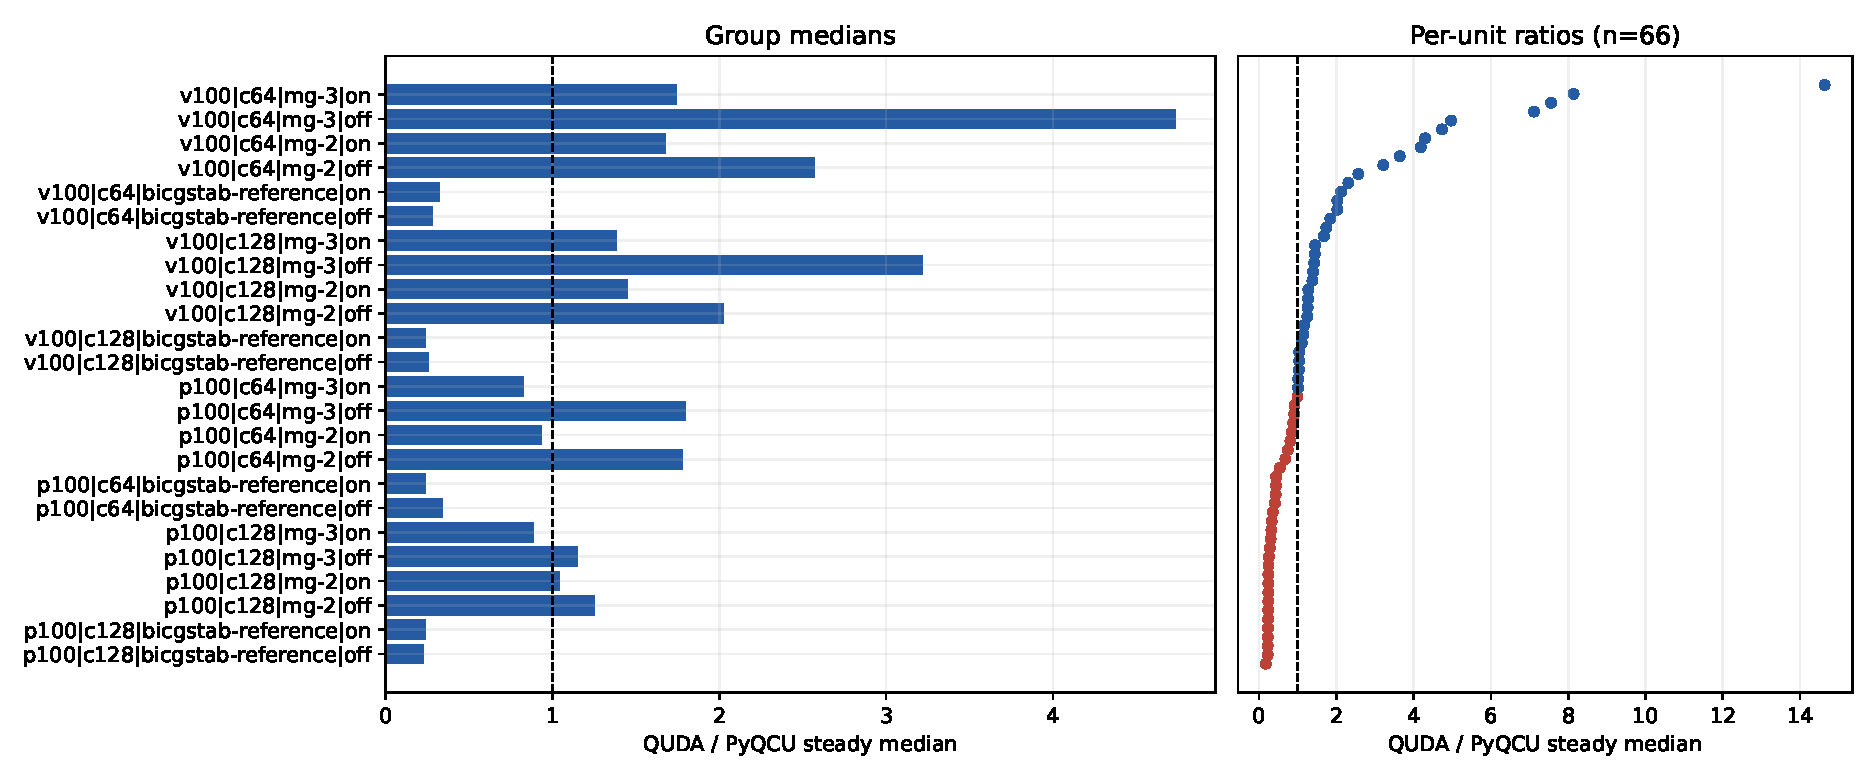
\includegraphics[width=0.98\linewidth,height=0.68\textheight,keepaspectratio]{overlap_matrix.pdf}
\caption{按设备、精度、求解器和 trace 模式分组的中位时间比。
$>1$ 表示 PyQCU/QUDA 的 steady median 比值有利于 PyQCU。}
\end{figure}

\section{构建与运行 provenance}

\begin{table}[htbp]
\centering
\caption{设备和二进制身份}
\small
\begin{tabularx}{\textwidth}{@{}L{0.18\textwidth}L{0.36\textwidth}Y@{}}
\toprule
设备 & 运行栈 & 二进制与架构 \\
\midrule
V100 & PyTorch 2.10.0+cu128；CUDA 12.8；PyQUDA 0.10.54 &
\path{cpp/cuda/qcu/libqcu.so}，SHA256
\code{81ec614211a50954...a670889}，\code{sm_70} cubin；
QUDA \code{quda-double-install}，\code{sm_70}，
QIO/QMP/MG-double/reconstruct 7 \\
P100 & PyTorch 2.7.1+cu118；CUDA 11.8；PyQUDA 0.10.54 &
\path{data/build/libqcu_arch/sm60/libqcu.so}，SHA256
\code{e29c1cf04a57ec3b...d0c20e1}，\code{sm_60} cubin；
QUDA \code{quda-sm60-install}，\code{sm_60}，
QIO/QMP/MG-double/reconstruct 7 \\
\bottomrule
\end{tabularx}
\end{table}

QUDA tuning cache 固定为 \path{data/quda-resource-sm70-20260927} 和
\path{data/quda-resource-sm60-20260927}。P100 使用
\code{2x1x1x1} process grid，一线程一卡；V100 使用单 rank。
QIO null-vector manifest 与二进制均放在 \path{data/qio-matrix}，
避免 manifest/artifact 分根造成的 fail-closed 阻塞。

\section{性能结果}

\subsection{分组中位时间比}

表中的比值为
\begin{equation}
 R = \frac{t_{\mathrm{QUDA,steady}}}{t_{\mathrm{PyQCU,steady}}}.
\end{equation}
$R>1$ 表示 PyQCU 更快。trace-on 数据包含诊断同步开销，只用于归因；
trace-off 数据用于正式性能判断。

\begin{longtable}{@{}llllrrrr@{}}
\caption{分组中位时间比（QUDA / PyQCU）}\label{tab:group-ratio}\\
\toprule
设备 & 精度 & 求解 & trace & 样本 & median & min & max \\
\midrule
\endfirsthead
\toprule
设备 & 精度 & 求解 & trace & 样本 & median & min & max \\
\midrule
\endhead
V100 & c64 & BiCGStab & off & 3 & 0.2818 & 0.2355 & 0.3288 \\
V100 & c64 & BiCGStab & on & 3 & 0.3213 & 0.1766 & 0.4102 \\
V100 & c64 & MG-2 & off & 3 & 2.5717 & 1.3999 & 7.1161 \\
V100 & c64 & MG-2 & on & 3 & 1.6785 & 1.0387 & 3.6403 \\
V100 & c64 & MG-3 & off & 3 & 4.7366 & 2.0284 & 8.1391 \\
V100 & c64 & MG-3 & on & 3 & 1.7444 & 1.2602 & 4.1878 \\
V100 & c128 & BiCGStab & off & 3 & 0.2580 & 0.2463 & 0.3573 \\
V100 & c128 & BiCGStab & on & 3 & 0.2397 & 0.2242 & 0.2998 \\
V100 & c128 & MG-2 & off & 3 & 2.0269 & 0.5401 & 7.5586 \\
V100 & c128 & MG-2 & on & 3 & 1.4515 & 1.0124 & 4.9719 \\
V100 & c128 & MG-3 & off & 3 & 3.2174 & 1.8447 & 14.6340 \\
V100 & c128 & MG-3 & on & 3 & 1.3822 & 0.9966 & 4.2991 \\
P100 & c64 & BiCGStab & off & 2 & 0.3416 & 0.2403 & 0.4429 \\
P100 & c64 & BiCGStab & on & 2 & 0.2368 & 0.2333 & 0.2404 \\
P100 & c64 & MG-2 & off & 2 & 1.7773 & 1.4305 & 2.1241 \\
P100 & c64 & MG-2 & on & 2 & 0.9341 & 0.8531 & 1.0150 \\
P100 & c64 & MG-3 & off & 2 & 1.7944 & 1.2758 & 2.3130 \\
P100 & c64 & MG-3 & on & 2 & 0.8282 & 0.7456 & 0.9107 \\
P100 & c128 & BiCGStab & off & 3 & 0.2284 & 0.2244 & 0.4334 \\
P100 & c128 & BiCGStab & on & 3 & 0.2400 & 0.2386 & 0.4383 \\
P100 & c128 & MG-2 & off & 3 & 1.2502 & 1.0349 & 1.2725 \\
P100 & c128 & MG-2 & on & 3 & 1.0420 & 0.8120 & 1.1716 \\
P100 & c128 & MG-3 & off & 3 & 1.1517 & 1.1061 & 1.4436 \\
P100 & c128 & MG-3 & on & 3 & 0.8843 & 0.6831 & 0.9181 \\
\bottomrule
\end{longtable}

所有精确单元的全矩阵中位比值 $R$ 为 1.0250，MG-2/3 共 35/44 个单元
优于 QUDA；BiCGStab 参考求解器为 0/22，QUDA 在各精确点上更快。
因此 MultiGrid 组的优势不能外推为 PyQCU 全部求解器优势。

\subsection{逐单元视图}

\begin{figure}[htbp]
\centering
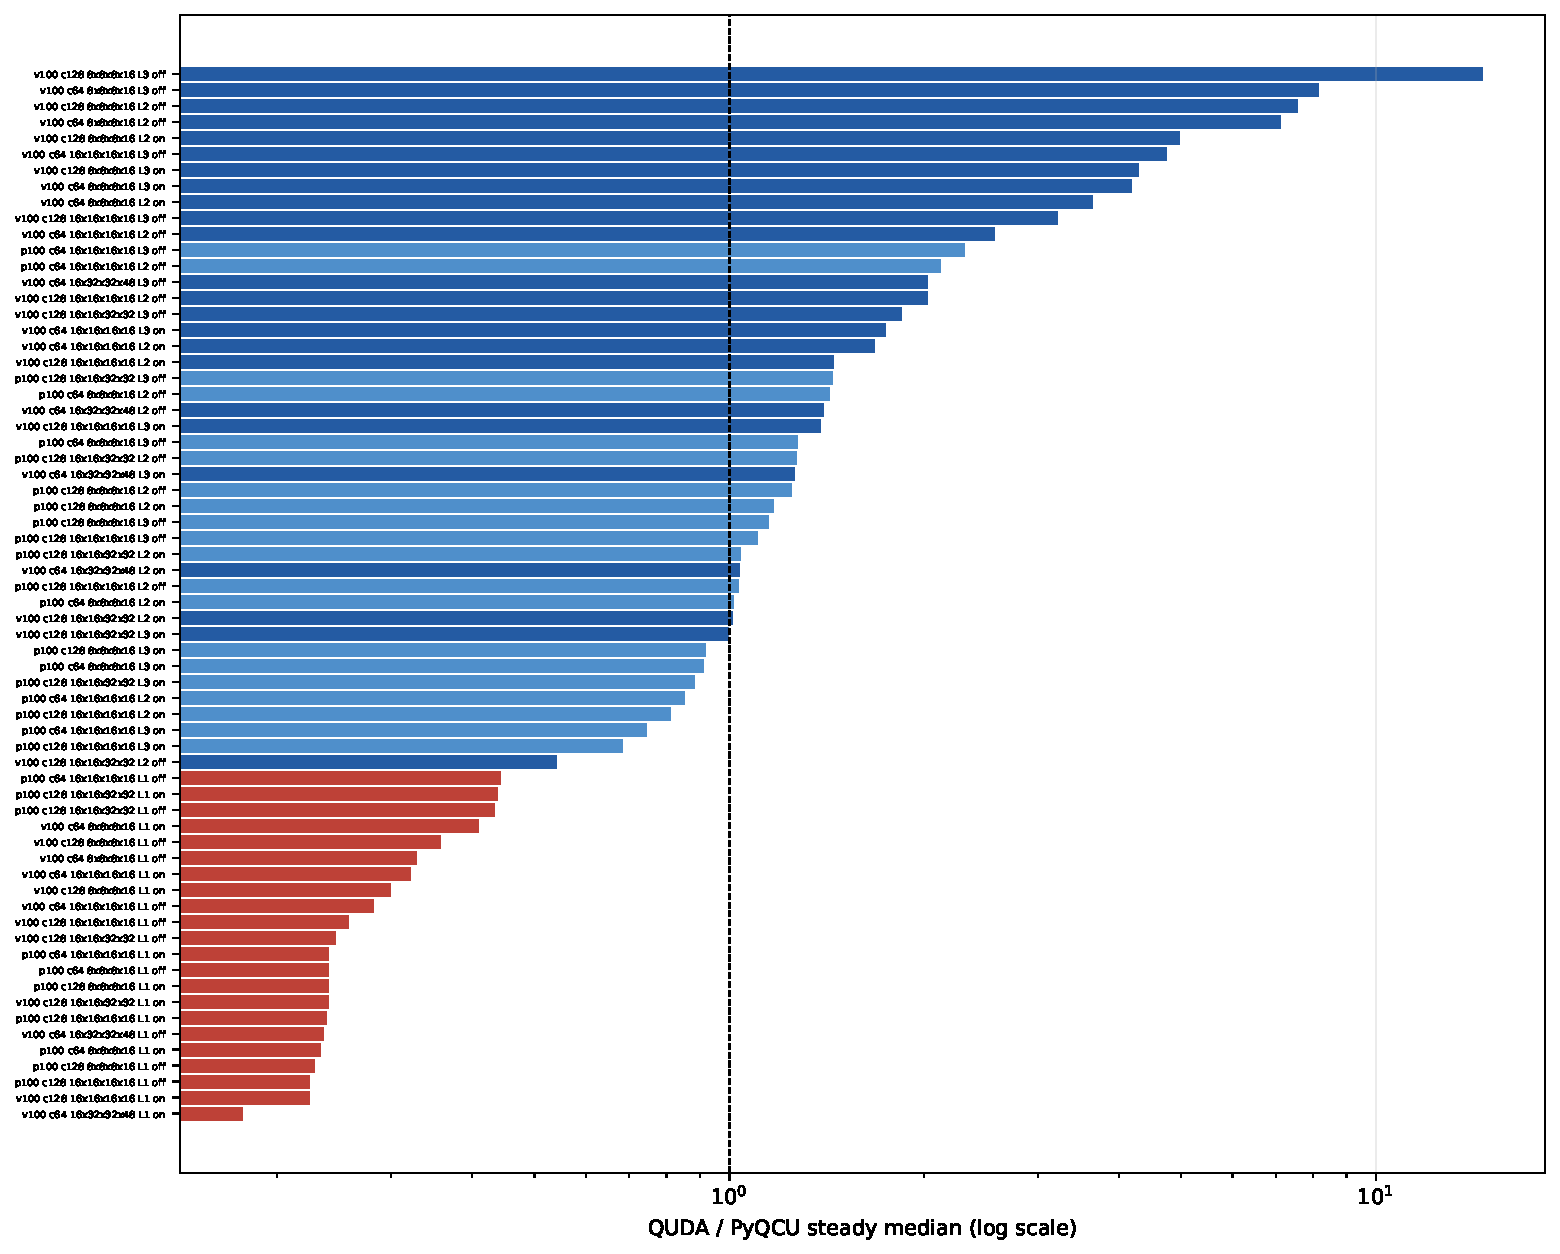
\includegraphics[width=0.98\linewidth,height=0.68\textheight,keepaspectratio]{mg_speedup_units.pdf}
\caption{66 个精确 combined 单元的逐单元时间比。}
\end{figure}

\begin{figure}[htbp]
\centering

\includegraphics[width=0.98\linewidth,height=0.68\textheight,keepaspectratio]{mg_speedup_device.pdf}
\caption{PyQCU/QUDA steady median、相对时间和设备标签。}
\end{figure}

\section{逐层分解与迭代}

\begin{figure}[htbp]
\centering
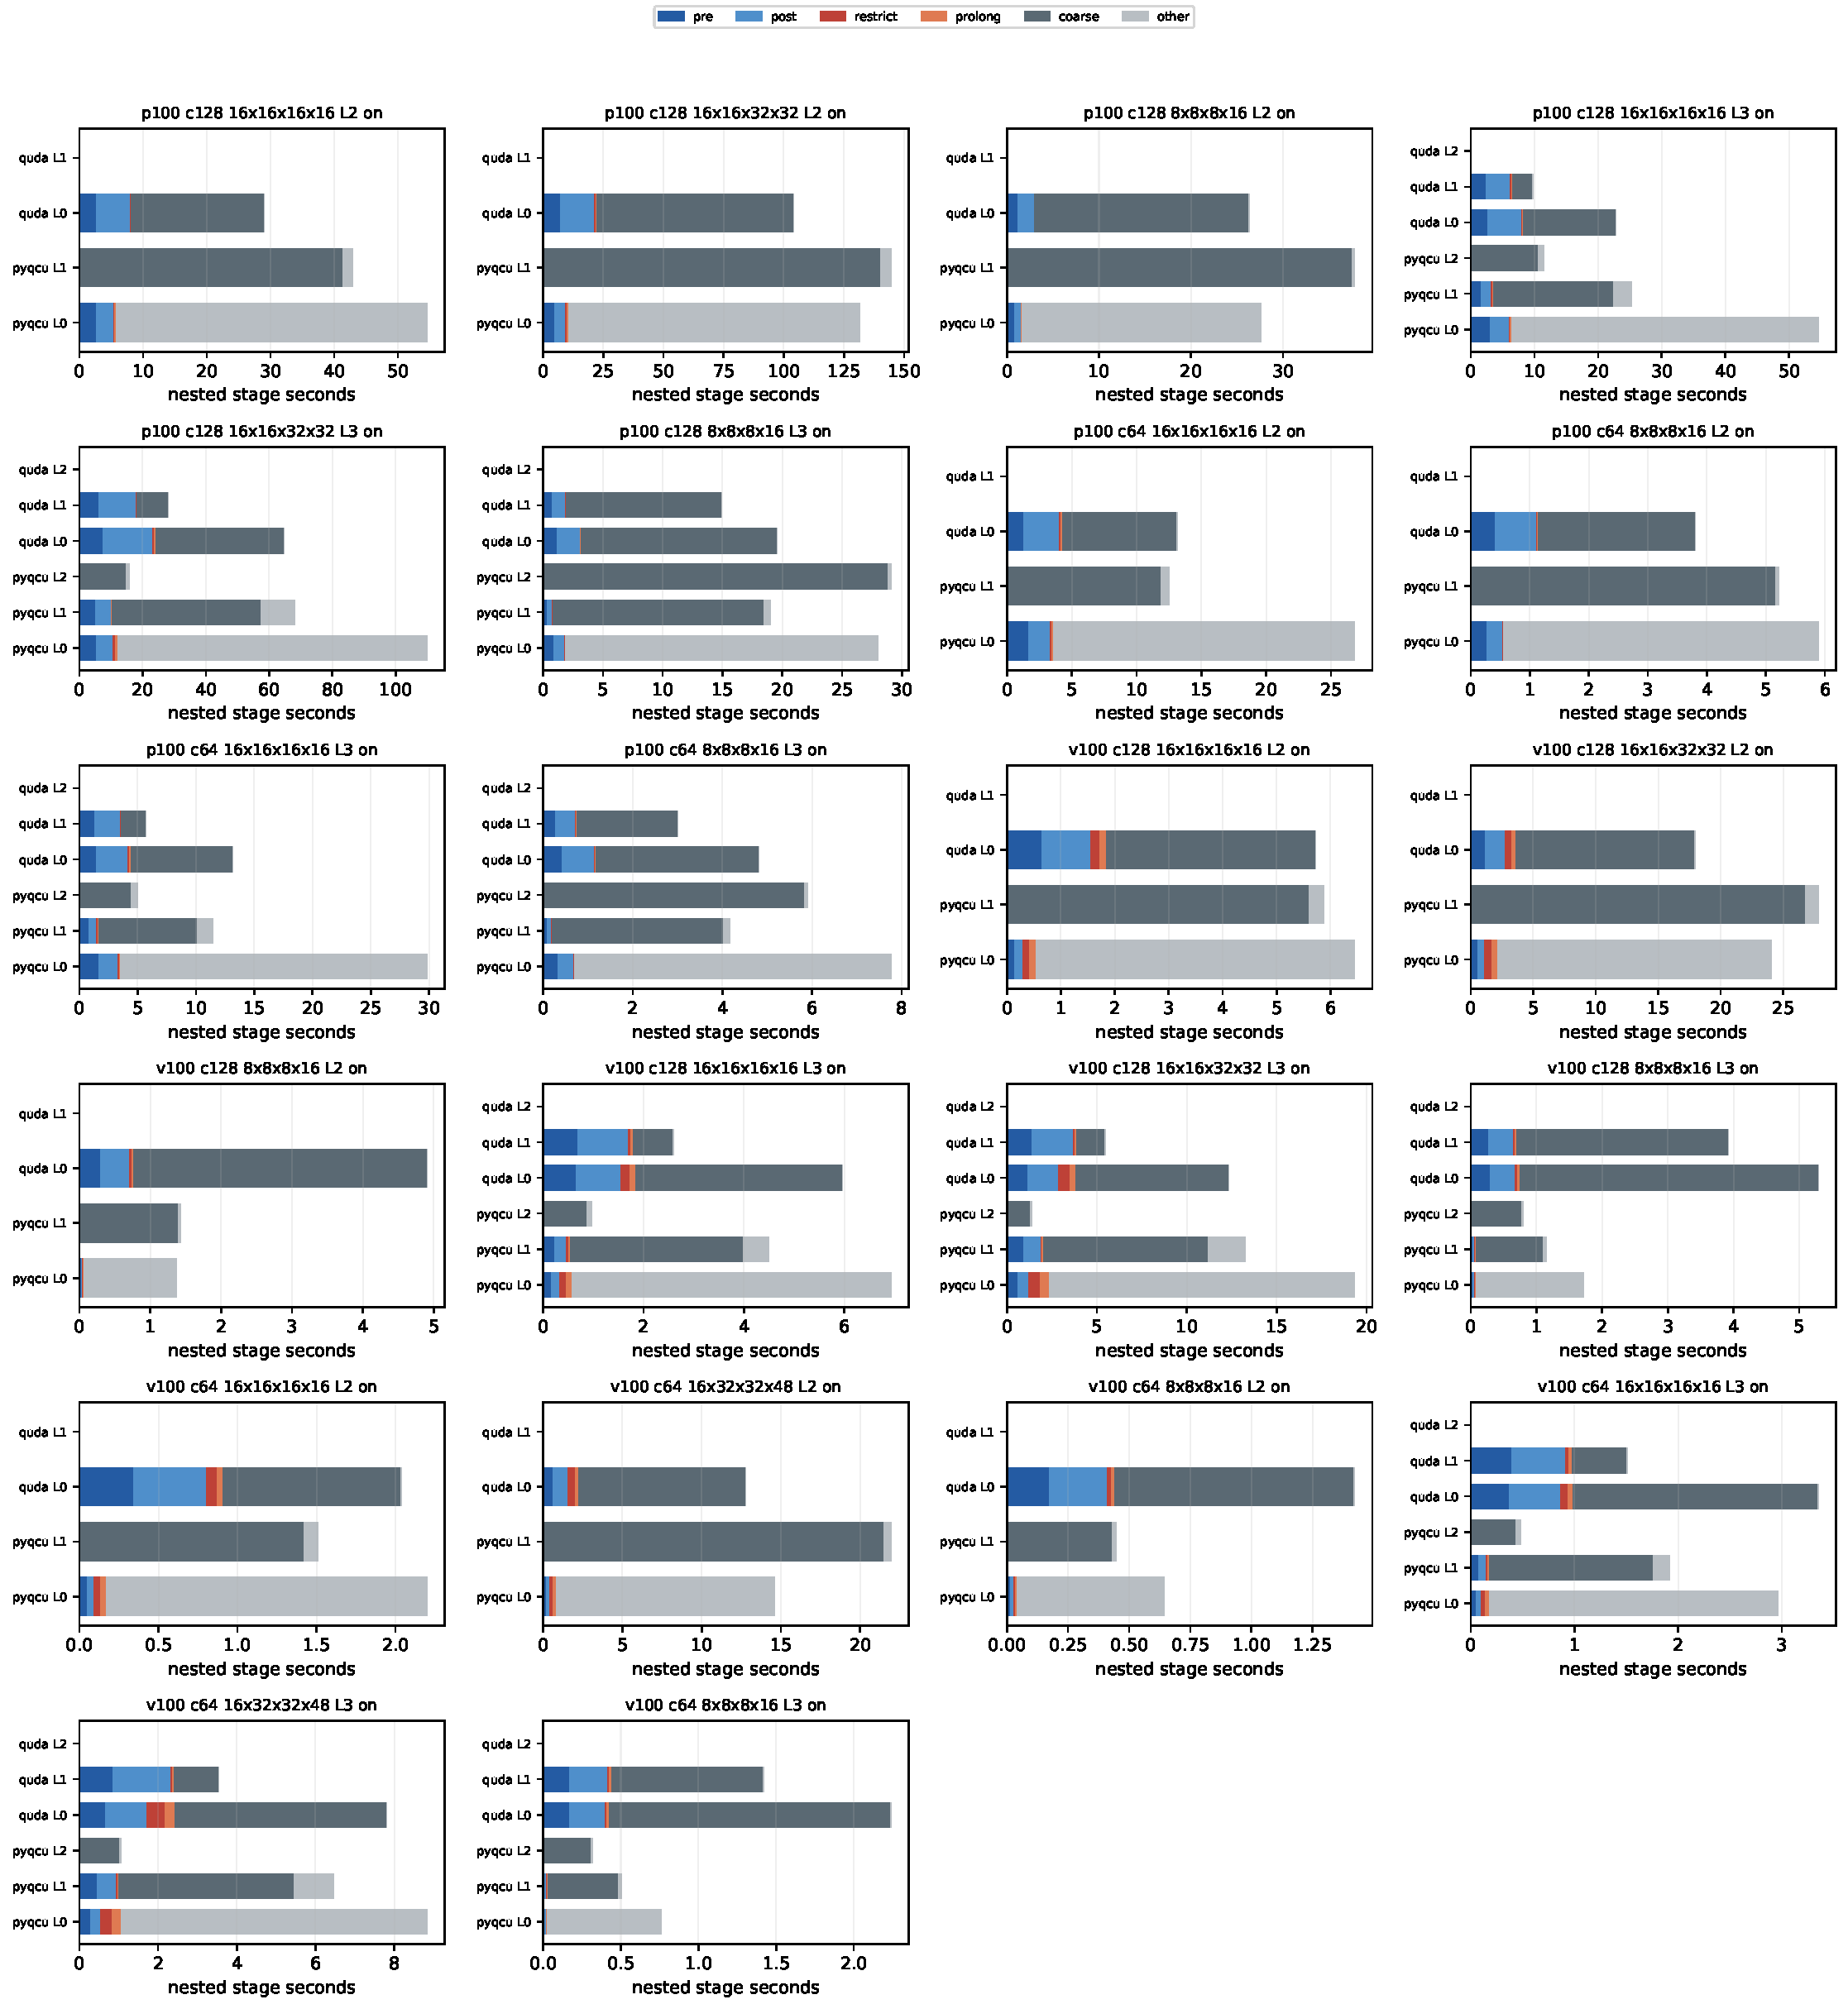
\includegraphics[width=0.98\linewidth,height=0.68\textheight,keepaspectratio]{mg_stage_breakdown.pdf}
\caption{全部 trace-on MG-2/3 的逐层 phase 堆叠分解；逐单元格精确
数值和迭代数见配套的 level/stage CSV。}
\end{figure}

精确单元的 phase、层级和迭代记录分别保存在
\path{mg_matrix.csv}、\path{mg_levels.csv} 与
\path{final_protocol/stages.csv}。最细层迭代数是外层 FGMRES/GCR
迭代数，不把 smoother 与 coarse solver 迭代相加。

\section{峰值显存}

下表使用每个 side-case 的不计时 device-wide sampler
\code{device_used_max_observed_bytes}；它可能包含测试进程之外的同设备
分配，因此用于门限检查，不声明为进程独占峰值。

\begin{table}[htbp]
\centering
\caption{峰值 device-wide 显存（MiB）}
\small
\begin{tabular}{@{}llrrr@{}}
\toprule
侧 & 设备/精度 & 样本 & median & max \\
\midrule
PyQCU & P100/c64 & 12 & 1852.9 & 2134.9 \\
PyQCU & P100/c128 & 18 & 3150.9 & 7308.9 \\
PyQCU & V100/c64 & 18 & 2677.3 & 11907.3 \\
PyQCU & V100/c128 & 18 & 4005.3 & 9575.3 \\
QUDA & P100/c64 & 12 & 1934.9 & 2628.9 \\
QUDA & P100/c128 & 18 & 3800.9 & 11082.9 \\
QUDA & V100/c64 & 18 & 3587.3 & 23063.3 \\
QUDA & V100/c128 & 18 & 5227.3 & 15739.3 \\
\bottomrule
\end{tabular}
\end{table}

\begin{figure}[htbp]
\centering
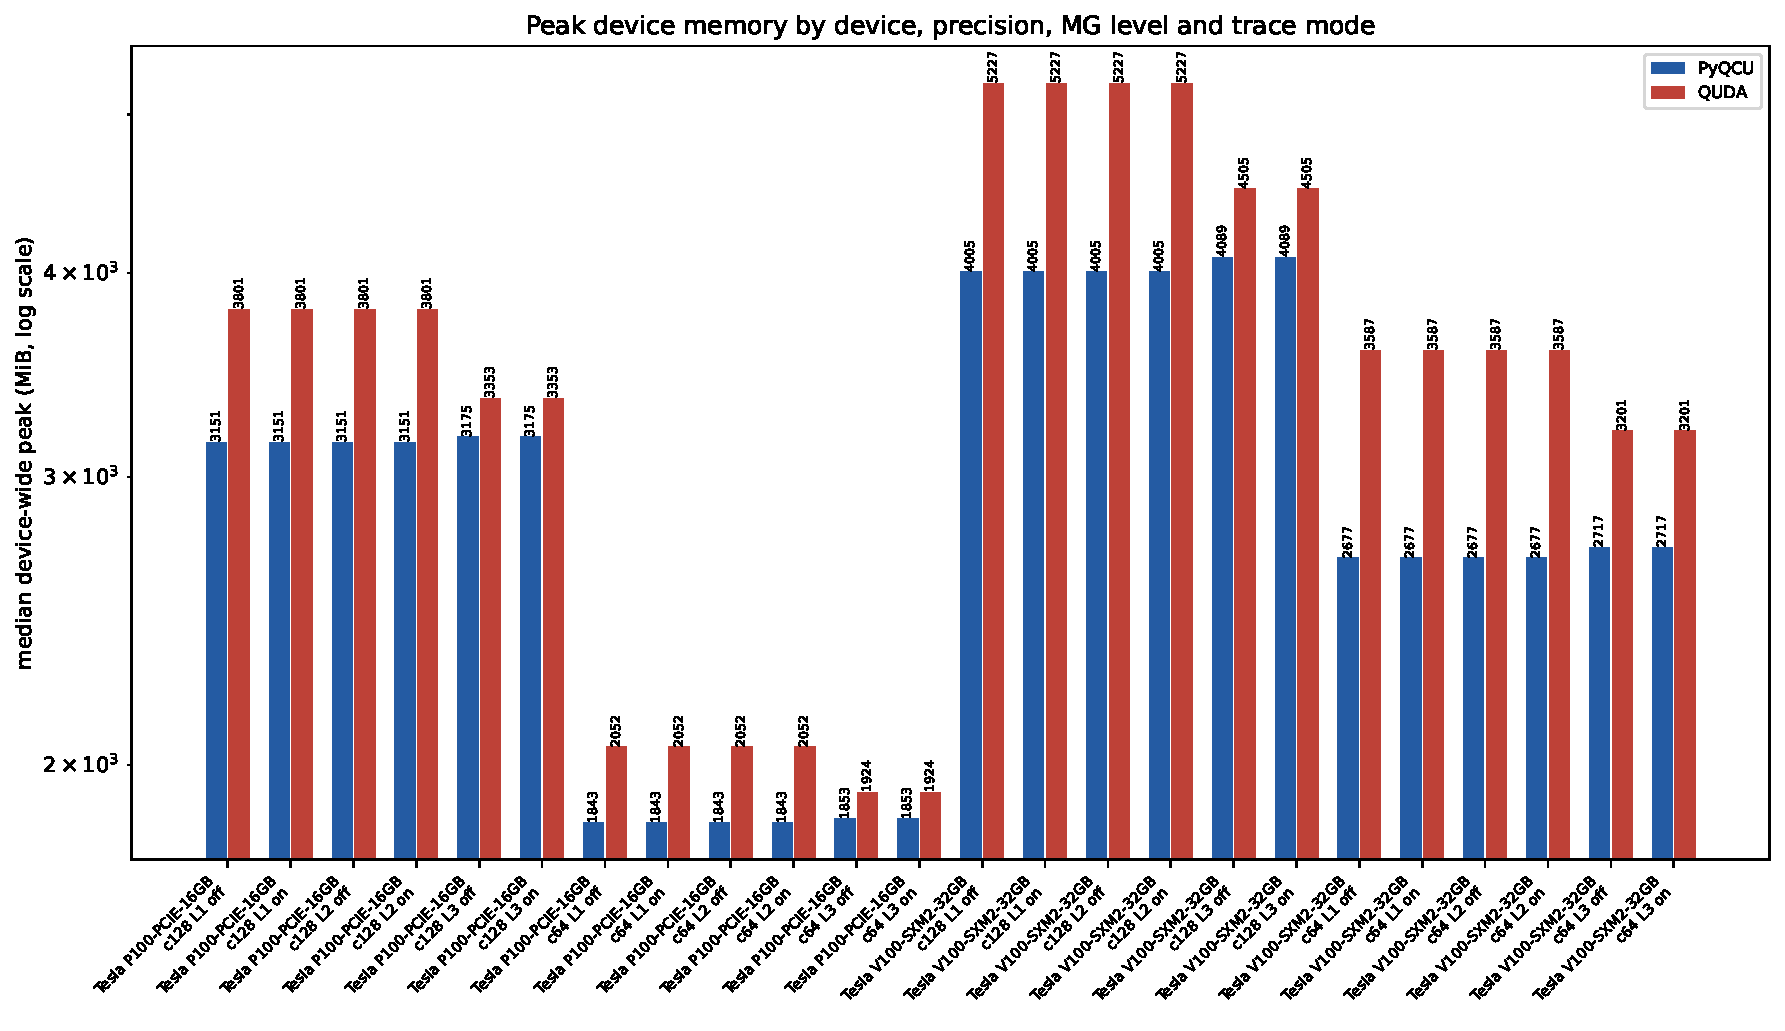
\includegraphics[width=0.98\linewidth,height=0.68\textheight,keepaspectratio]{mg_peak_memory.pdf}
\caption{设备级峰值显存按设备、精度、MG 层数和 trace 模式的中位数。}
\end{figure}

精确单元中最大的 PyQCU 观测峰值约 11.9 GiB（V100 36.3\%），最大 QUDA
观测峰值约 23.1 GiB（V100 70.4\%）。所有保留的精确结果均低于 85\%
显存门限。逐 side、setup、first solve、steady、allocator 与 workspace
原值见 \path{mg_memory.csv}。

\section{残差收敛}

\begin{table}[htbp]
\centering
\caption{稳态最细层 full true residual}
\small
\begin{tabular}{@{}lrrr@{}}
\toprule
侧 & 样本 & median & max \\
\midrule
PyQCU & 66 & $1.85\times10^{-8}$ & $7.40\times10^{-7}$ \\
QUDA & 66 & $1.89\times10^{-8}$ & $7.97\times10^{-7}$ \\
\bottomrule
\end{tabular}
\end{table}

\begin{figure}[htbp]
\centering
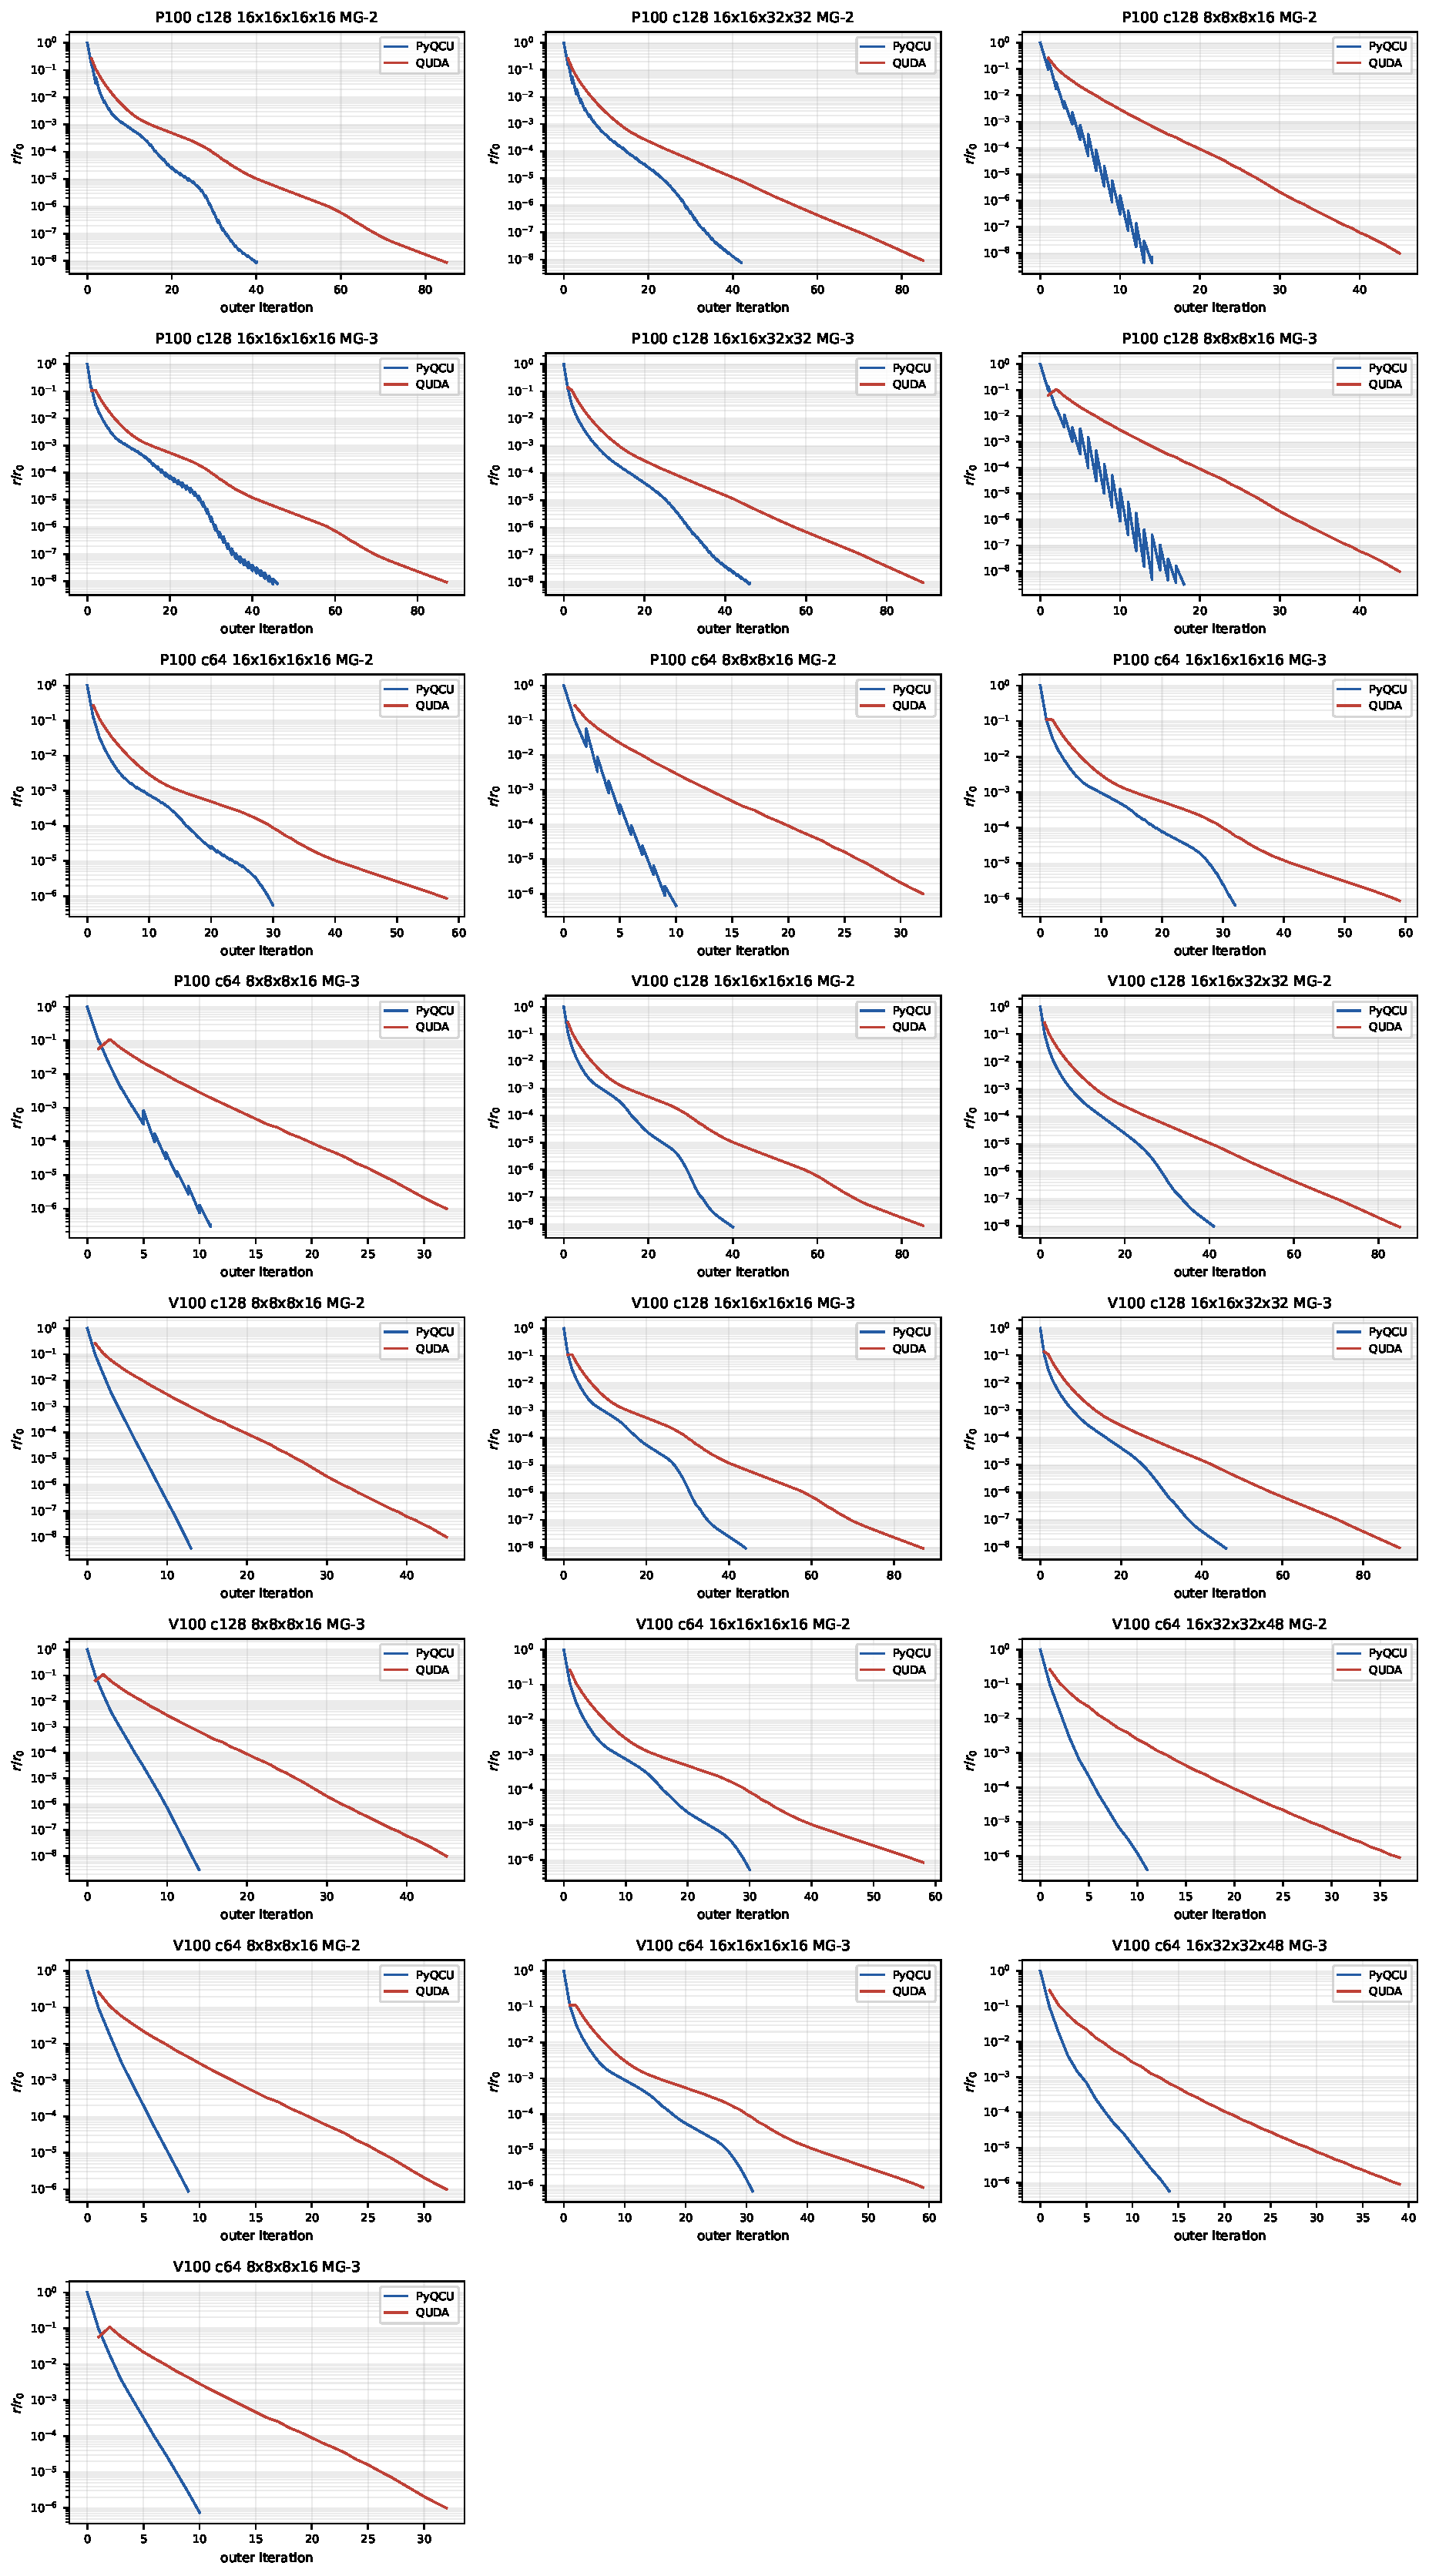
\includegraphics[width=0.98\linewidth,height=0.68\textheight,keepaspectratio]{mg_residual_curves.pdf}
\caption{全部 44 个 trace-on MG-2/3 side 的最细层收敛曲线。}
\end{figure}

\begin{figure}[htbp]
\centering
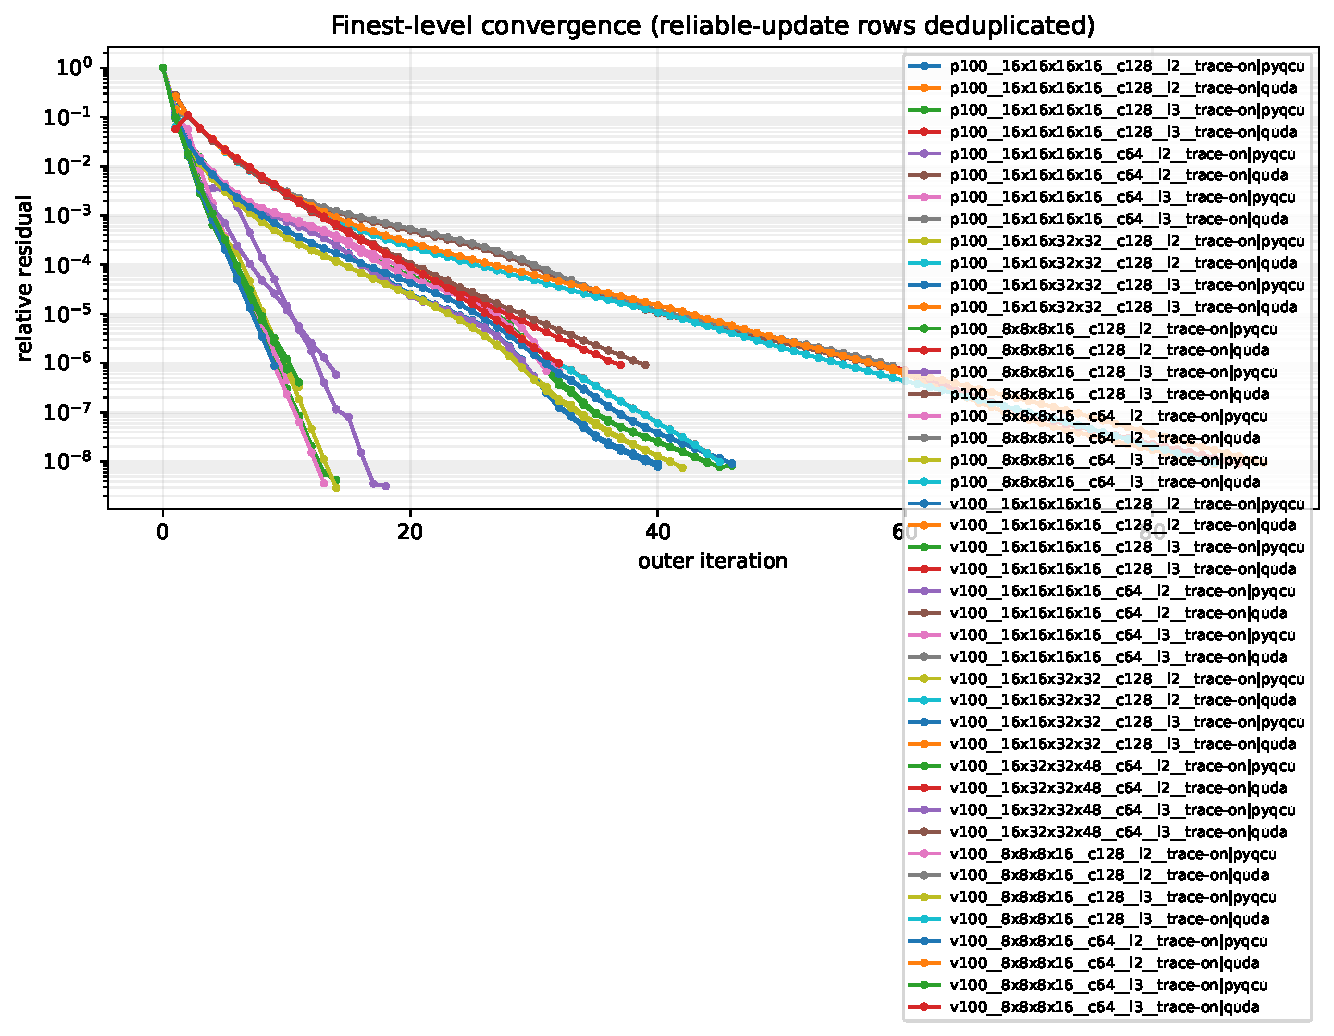
\includegraphics[width=0.98\linewidth,height=0.68\textheight,keepaspectratio]{mg_finest_residual.pdf}
\caption{最细层残差总览。}
\end{figure}

两次递推标量的定义不同：PyQCU 主要记录 Arnoldi least-squares estimate，
QUDA 记录 GCR iterated residual；因此曲线可用于观察下降趋势，但最终
通过与否只由独立 full-operator true residual 判定。

\section{容量替代记录}

双 P100 的 $16\times32\times32\times48$ c64 请求项三次尝试均未同时满足
资源与时间门限：默认路径峰值约 15.9 GiB；\code{PYQCU_MPI_OVERLAP=0}
约 14.8 GiB；extended CPU-staging 路径约 12.4 GiB，但 MG-2 setup 仍
超过 570 秒。该 6 个 combined 项因此映射到已完整实测的 $16^4$ c64
对应项，并在 \path{capacity_substitutions.csv} 中显式标识。

\begin{table}[htbp]
\centering
\caption{容量替代项}\label{tab:capacity-substitution}
\small
\begin{tabularx}{\textwidth}{@{}L{0.27\textwidth}L{0.27\textwidth}L{0.13\textwidth}Y@{}}
\toprule
请求单元 & 有效单元 & 状态 & 原因 \\
\midrule
\path{p100__16x32x32x48__c64__l1__trace-off} &
\path{p100__16x16x16x16__c64__l1__trace-off} & substituted &
显存/时限 \\
\path{p100__16x32x32x48__c64__l1__trace-on} &
\path{p100__16x16x16x16__c64__l1__trace-on} & substituted &
显存/时限 \\
\path{p100__16x32x32x48__c64__l2__trace-off} &
\path{p100__16x16x16x16__c64__l2__trace-off} & substituted &
显存/时限 \\
\path{p100__16x32x32x48__c64__l2__trace-on} &
\path{p100__16x16x16x16__c64__l2__trace-on} & substituted &
显存/时限 \\
\path{p100__16x32x32x48__c64__l3__trace-off} &
\path{p100__16x16x16x16__c64__l3__trace-off} & substituted &
显存/时限 \\
\path{p100__16x32x32x48__c64__l3__trace-on} &
\path{p100__16x16x16x16__c64__l3__trace-on} & substituted &
显存/时限 \\
\bottomrule
\end{tabularx}
\end{table}

替代项只作为容量趋势证据，不得和原大格的公平加速比混合。完整中止
记录见 \path{capacity_guard_events.json}。

\section{结论}

\begin{enumerate}
  \item 在本轮 66 个精确格点上，PyQCU MG-2/3 的稳态中位时间比在多数
        V100 组显著大于 1，尤以 V100 c64 MG-3 trace-off 的
        $4.74\times$ 和 c128 MG-3 trace-off 的 $3.22\times$ 最明显；
        但 c128 最大单点达到 $14.63\times$，说明结果对格点与残差轨迹
        敏感，不能外推为普遍优势。
  \item 双 P100 上 MG-2/3 的优势主要出现在 trace-off；trace-on 的诊断
        同步使 PyQCU 比值下降，部分组退到 1 以下。正式性能结论必须
        使用 trace-off。
  \item QUDA BiCGStab 在全部 22 个精确参考点更快，故 MultiGrid 对照
        不能替代总求解器结论。
  \item 所有保留精确结果的 PyQCU/QUDA 真残差最大值分别为
        $7.40\times10^{-7}$ 与 $7.97\times10^{-7}$，均通过
        $5\times10^{-6}$ 门限。
  \item 保留样本均低于 85\% 显存门限；P100 c64 大格只有在性能 setup
        超过 570 秒时才被明确替代，未发生静默跳过。
\end{enumerate}

\section{复现与原始证据}

\begin{verbatim}
data/mg_matrix_comprehensive_final_20260928/
  matrix_state.jsonl
  units/*.json
  combined/*.json
  capacity_substitutions.json
  capacity_guard_events.json

data/report_multigrid_comprehensive_20260928/final_protocol/
  units.csv
  stages.csv
  references.csv
  overlap_matrix.{csv,svg,pdf}
  capacity_substitutions.csv
  requested_matrix_status.csv
  report/mg_matrix.csv
  report/mg_levels.csv
  report/mg_memory.csv
  report/*.svg
  report/*.pdf
\end{verbatim}

主矩阵命令为
\path{pyqcu/testing/qcu/strict/quda_comparison/bench_mg_matrix_full.py}，
侧记录生成器为
\path{pyqcu/testing/qcu/strict/quda_comparison/bench_strict_vs_quda.py}，
合并与审计器为
\path{pyqcu/testing/qcu/strict/quda_comparison/assemble_final_matrix.py}，
图表和表格生成器为
\path{pyqcu/testing/qcu/strict/quda_comparison/build_mg_report.py}。

\end{document}
